\PassOptionsToPackage{unicode=true}{hyperref} % options for packages loaded elsewhere
\PassOptionsToPackage{hyphens}{url}
%
\documentclass[
]{article}
\usepackage{lmodern}
\usepackage{amssymb,amsmath}
\usepackage{ifxetex,ifluatex}
\ifnum 0\ifxetex 1\fi\ifluatex 1\fi=0 % if pdftex
  \usepackage[T1]{fontenc}
  \usepackage[utf8]{inputenc}
  \usepackage{textcomp} % provides euro and other symbols
\else % if luatex or xelatex
  \usepackage{unicode-math}
  \defaultfontfeatures{Scale=MatchLowercase}
  \defaultfontfeatures[\rmfamily]{Ligatures=TeX,Scale=1}
\fi
% use upquote if available, for straight quotes in verbatim environments
\IfFileExists{upquote.sty}{\usepackage{upquote}}{}
\IfFileExists{microtype.sty}{% use microtype if available
  \usepackage[]{microtype}
  \UseMicrotypeSet[protrusion]{basicmath} % disable protrusion for tt fonts
}{}
\makeatletter
\@ifundefined{KOMAClassName}{% if non-KOMA class
  \IfFileExists{parskip.sty}{%
    \usepackage{parskip}
  }{% else
    \setlength{\parindent}{0pt}
    \setlength{\parskip}{6pt plus 2pt minus 1pt}}
}{% if KOMA class
  \KOMAoptions{parskip=half}}
\makeatother
\usepackage{xcolor}
\IfFileExists{xurl.sty}{\usepackage{xurl}}{} % add URL line breaks if available
\IfFileExists{bookmark.sty}{\usepackage{bookmark}}{\usepackage{hyperref}}
\hypersetup{
  pdftitle={ExampleOfSignatureQBiC},
  pdfauthor={Mo Liu, Steven G. Rozen},
  pdfborder={0 0 0},
  breaklinks=true}
\urlstyle{same}  % don't use monospace font for urls
\usepackage[margin=1in]{geometry}
\usepackage{color}
\usepackage{fancyvrb}
\newcommand{\VerbBar}{|}
\newcommand{\VERB}{\Verb[commandchars=\\\{\}]}
\DefineVerbatimEnvironment{Highlighting}{Verbatim}{commandchars=\\\{\}}
% Add ',fontsize=\small' for more characters per line
\usepackage{framed}
\definecolor{shadecolor}{RGB}{248,248,248}
\newenvironment{Shaded}{\begin{snugshade}}{\end{snugshade}}
\newcommand{\AlertTok}[1]{\textcolor[rgb]{0.94,0.16,0.16}{#1}}
\newcommand{\AnnotationTok}[1]{\textcolor[rgb]{0.56,0.35,0.01}{\textbf{\textit{#1}}}}
\newcommand{\AttributeTok}[1]{\textcolor[rgb]{0.77,0.63,0.00}{#1}}
\newcommand{\BaseNTok}[1]{\textcolor[rgb]{0.00,0.00,0.81}{#1}}
\newcommand{\BuiltInTok}[1]{#1}
\newcommand{\CharTok}[1]{\textcolor[rgb]{0.31,0.60,0.02}{#1}}
\newcommand{\CommentTok}[1]{\textcolor[rgb]{0.56,0.35,0.01}{\textit{#1}}}
\newcommand{\CommentVarTok}[1]{\textcolor[rgb]{0.56,0.35,0.01}{\textbf{\textit{#1}}}}
\newcommand{\ConstantTok}[1]{\textcolor[rgb]{0.00,0.00,0.00}{#1}}
\newcommand{\ControlFlowTok}[1]{\textcolor[rgb]{0.13,0.29,0.53}{\textbf{#1}}}
\newcommand{\DataTypeTok}[1]{\textcolor[rgb]{0.13,0.29,0.53}{#1}}
\newcommand{\DecValTok}[1]{\textcolor[rgb]{0.00,0.00,0.81}{#1}}
\newcommand{\DocumentationTok}[1]{\textcolor[rgb]{0.56,0.35,0.01}{\textbf{\textit{#1}}}}
\newcommand{\ErrorTok}[1]{\textcolor[rgb]{0.64,0.00,0.00}{\textbf{#1}}}
\newcommand{\ExtensionTok}[1]{#1}
\newcommand{\FloatTok}[1]{\textcolor[rgb]{0.00,0.00,0.81}{#1}}
\newcommand{\FunctionTok}[1]{\textcolor[rgb]{0.00,0.00,0.00}{#1}}
\newcommand{\ImportTok}[1]{#1}
\newcommand{\InformationTok}[1]{\textcolor[rgb]{0.56,0.35,0.01}{\textbf{\textit{#1}}}}
\newcommand{\KeywordTok}[1]{\textcolor[rgb]{0.13,0.29,0.53}{\textbf{#1}}}
\newcommand{\NormalTok}[1]{#1}
\newcommand{\OperatorTok}[1]{\textcolor[rgb]{0.81,0.36,0.00}{\textbf{#1}}}
\newcommand{\OtherTok}[1]{\textcolor[rgb]{0.56,0.35,0.01}{#1}}
\newcommand{\PreprocessorTok}[1]{\textcolor[rgb]{0.56,0.35,0.01}{\textit{#1}}}
\newcommand{\RegionMarkerTok}[1]{#1}
\newcommand{\SpecialCharTok}[1]{\textcolor[rgb]{0.00,0.00,0.00}{#1}}
\newcommand{\SpecialStringTok}[1]{\textcolor[rgb]{0.31,0.60,0.02}{#1}}
\newcommand{\StringTok}[1]{\textcolor[rgb]{0.31,0.60,0.02}{#1}}
\newcommand{\VariableTok}[1]{\textcolor[rgb]{0.00,0.00,0.00}{#1}}
\newcommand{\VerbatimStringTok}[1]{\textcolor[rgb]{0.31,0.60,0.02}{#1}}
\newcommand{\WarningTok}[1]{\textcolor[rgb]{0.56,0.35,0.01}{\textbf{\textit{#1}}}}
\usepackage{graphicx,grffile}
\makeatletter
\def\maxwidth{\ifdim\Gin@nat@width>\linewidth\linewidth\else\Gin@nat@width\fi}
\def\maxheight{\ifdim\Gin@nat@height>\textheight\textheight\else\Gin@nat@height\fi}
\makeatother
% Scale images if necessary, so that they will not overflow the page
% margins by default, and it is still possible to overwrite the defaults
% using explicit options in \includegraphics[width, height, ...]{}
\setkeys{Gin}{width=\maxwidth,height=\maxheight,keepaspectratio}
\setlength{\emergencystretch}{3em}  % prevent overfull lines
\providecommand{\tightlist}{%
  \setlength{\itemsep}{0pt}\setlength{\parskip}{0pt}}
\setcounter{secnumdepth}{-2}
% Redefines (sub)paragraphs to behave more like sections
\ifx\paragraph\undefined\else
  \let\oldparagraph\paragraph
  \renewcommand{\paragraph}[1]{\oldparagraph{#1}\mbox{}}
\fi
\ifx\subparagraph\undefined\else
  \let\oldsubparagraph\subparagraph
  \renewcommand{\subparagraph}[1]{\oldsubparagraph{#1}\mbox{}}
\fi

% set default figure placement to htbp
\makeatletter
\def\fps@figure{htbp}
\makeatother


\title{ExampleOfSignatureQBiC}
\author{Mo Liu, Steven G. Rozen}
\date{12/30/2020}

\begin{document}
\maketitle

\hypertarget{example-of-signature-qbic-for-hoxd13-and-mutational-signature-sbs7a}{%
\subsection{Example of Signature-QBiC for HOXD13 and mutational
signature
SBS7a}\label{example-of-signature-qbic-for-hoxd13-and-mutational-signature-sbs7a}}

This is the example shown in Figure 1b of Liu et al., Mutational
Processes in Cancer Preferentially Affect Binding of Particular
Transcription Factors.

\hypertarget{load-libraries}{%
\subsection{Load libraries}\label{load-libraries}}

\begin{Shaded}
\begin{Highlighting}[]
\KeywordTok{library}\NormalTok{(PCAWG7)}
\KeywordTok{library}\NormalTok{(tibble)}
\KeywordTok{library}\NormalTok{(knitr)}
\end{Highlighting}
\end{Shaded}

\begin{Shaded}
\begin{Highlighting}[]
\NormalTok{PCAWG_subs_signature <-}\StringTok{ }\NormalTok{PCAWG7}\OperatorTok{::}\NormalTok{signature}\OperatorTok{$}\NormalTok{genome}\OperatorTok{$}\NormalTok{SBS96}

\NormalTok{mut.types <-}\StringTok{ }\KeywordTok{lapply}\NormalTok{(}\KeywordTok{row.names}\NormalTok{(PCAWG_subs_signature),}\ControlFlowTok{function}\NormalTok{(x)\{}
  \KeywordTok{return}\NormalTok{(}\KeywordTok{paste}\NormalTok{(}\KeywordTok{substring}\NormalTok{(x,}\DecValTok{1}\NormalTok{,}\DecValTok{3}\NormalTok{),}
               \KeywordTok{paste}\NormalTok{(}\KeywordTok{substring}\NormalTok{(x,}\DecValTok{1}\NormalTok{,}\DecValTok{1}\NormalTok{),}
                     \KeywordTok{substring}\NormalTok{(x,}\DecValTok{4}\NormalTok{,}\DecValTok{4}\NormalTok{),}
                     \KeywordTok{substring}\NormalTok{(x,}\DecValTok{3}\NormalTok{,}\DecValTok{3}\NormalTok{),}\DataTypeTok{sep=}\StringTok{""}\NormalTok{),}
               \DataTypeTok{sep=}\StringTok{"_"}\NormalTok{))}
\NormalTok{\})}
\NormalTok{mut.types <-}\StringTok{ }\KeywordTok{row.names}\NormalTok{(PCAWG_subs_signature) <-}\StringTok{ }\KeywordTok{unlist}\NormalTok{(mut.types)}

\NormalTok{signature <-}\StringTok{ "SBS7a"} \CommentTok{##we used SBS7a as an example}
\NormalTok{sig <-}\StringTok{ }\NormalTok{PCAWG_subs_signature[ , signature, drop =}\StringTok{ }\OtherTok{FALSE}\NormalTok{]}

\NormalTok{all.possible.twelvemers <-}\StringTok{ }
\StringTok{  }\KeywordTok{tibble}\NormalTok{(}\KeywordTok{readRDS}\NormalTok{(}\StringTok{"../data-raw/all.possible.twelvemers.rds"}\NormalTok{)) }\CommentTok{##all mutations based on 11mers}
\end{Highlighting}
\end{Shaded}

Plotting function for Figure1

\begin{Shaded}
\begin{Highlighting}[]
\NormalTok{TruncatedHist <-}\StringTok{ }\ControlFlowTok{function}\NormalTok{(all.QBiC.scores,original.scores,weighted.prop,mutation.type)\{}
\NormalTok{  cut_off <-}\StringTok{ }\KeywordTok{quantile}\NormalTok{(all.QBiC.scores,}\KeywordTok{seq}\NormalTok{(}\DecValTok{0}\NormalTok{,}\DecValTok{1}\NormalTok{,}\FloatTok{0.01}\NormalTok{))[}\DecValTok{100}\NormalTok{] }\CommentTok{##pile the 1% tail up}
\NormalTok{  original.scores[original.scores}\OperatorTok{>}\NormalTok{cut_off] <-}\StringTok{ }\NormalTok{cut_off}
\NormalTok{  original.scores[original.scores}\OperatorTok{<}\NormalTok{(}\OperatorTok{-}\NormalTok{cut_off)] <-}\StringTok{ }\NormalTok{(}\OperatorTok{-}\NormalTok{cut_off)}
\NormalTok{  weighted.hist <-}\StringTok{ }\NormalTok{original.hist <-}\StringTok{ }\KeywordTok{hist}\NormalTok{(original.scores, }\DataTypeTok{breaks =} \KeywordTok{seq}\NormalTok{(}\OperatorTok{-}\NormalTok{(cut_off}\FloatTok{+0.5}\NormalTok{),}
\NormalTok{                                                                       (cut_off}\FloatTok{+0.5}\NormalTok{),}\FloatTok{0.5}\NormalTok{), }\DataTypeTok{plot=}\NormalTok{F)}
\NormalTok{  weighted.hist}\OperatorTok{$}\NormalTok{density <-}\StringTok{  }\NormalTok{weighted.hist}\OperatorTok{$}\NormalTok{density}\OperatorTok{*}\NormalTok{weighted.prop}
  \KeywordTok{plot}\NormalTok{(original.hist,}\DataTypeTok{freq =}\NormalTok{ F,}\DataTypeTok{ylim=}\KeywordTok{c}\NormalTok{(}\DecValTok{0}\NormalTok{,}\KeywordTok{max}\NormalTok{(original.hist}\OperatorTok{$}\NormalTok{density)}\OperatorTok{+}\FloatTok{0.05}\NormalTok{),}
       \DataTypeTok{main=}\KeywordTok{paste0}\NormalTok{(}\StringTok{"Original "}\NormalTok{,mutation.type),}\DataTypeTok{xaxt=}\StringTok{"n"}\NormalTok{,}\DataTypeTok{yaxt=}\StringTok{"n"}\NormalTok{)}
  \KeywordTok{plot}\NormalTok{(weighted.hist,}\DataTypeTok{freq=}\NormalTok{F,}\DataTypeTok{ylim =} \KeywordTok{c}\NormalTok{(}\DecValTok{0}\NormalTok{,}\KeywordTok{max}\NormalTok{(original.hist}\OperatorTok{$}\NormalTok{density)}\OperatorTok{+}\FloatTok{0.05}\NormalTok{),}
       \DataTypeTok{main=}\KeywordTok{paste0}\NormalTok{(}\StringTok{"Weighted "}\NormalTok{,mutation.type),}\DataTypeTok{xaxt=}\StringTok{"n"}\NormalTok{,}\DataTypeTok{yaxt=}\StringTok{"n"}\NormalTok{)}
\NormalTok{\}}
\end{Highlighting}
\end{Shaded}

The SignatureQBiC function. This function can also be found in SigQBiC
package. In SigQBiC package, SignatureQBiC function returns Gain Ratio
and Loss Ratio with the given QBiC scores, pvalues and signature. For
tutorial purpose, we split them into several chunks to show how we
calculate Gain Ratio and Loss Ratio. Therefore, the SignatureQBiC here
is slightly different from the one in package.

\begin{Shaded}
\begin{Highlighting}[]
\NormalTok{SignatureQBiC <-}\StringTok{ }\ControlFlowTok{function}\NormalTok{(QBiC_score_file_path,}
\NormalTok{                          pvalue_file_path,}
\NormalTok{                          sig, }
                          \DataTypeTok{plot.path =} \OtherTok{NULL}\NormalTok{) \{}
  
\NormalTok{  QBiC_scores_table <-}\StringTok{ }
\StringTok{    }\NormalTok{data.table}\OperatorTok{::}\KeywordTok{fread}\NormalTok{(QBiC_score_file_path,}
                      \DataTypeTok{sep=}\StringTok{" "}\NormalTok{, }\DataTypeTok{header=}\NormalTok{T, }\DataTypeTok{stringsAsFactors =}\NormalTok{ F, }\DataTypeTok{fill =}\NormalTok{ T)}
  \CommentTok{# This gives a data frame with colums diff and z_score}
  \CommentTok{# QBiC_scores_table contains NA for non-mutations, e.g AAAAAAAAAAA -> AAAAAAAAAAA}
  
\NormalTok{  pvalue <-}\StringTok{ }
\StringTok{    }\KeywordTok{scan}\NormalTok{(pvalue_file_path)}
  \CommentTok{# pvalue also contains NA for non-mutations}
\NormalTok{  pvalue <-}\StringTok{ }\NormalTok{pvalue[}\OperatorTok{!}\KeywordTok{is.na}\NormalTok{(pvalue)]}
  
\NormalTok{  QBiC_scores_matrix <-}\StringTok{ }
\StringTok{    }\KeywordTok{tibble}\NormalTok{(}\DataTypeTok{QBiC_mut =}\NormalTok{ all.possible.twelvemers}\OperatorTok{$}\NormalTok{seq, }
           \DataTypeTok{mut_type =}\NormalTok{ all.possible.twelvemers}\OperatorTok{$}\NormalTok{final_signature, }
           \DataTypeTok{scores   =}\NormalTok{ QBiC_scores_table}\OperatorTok{$}\NormalTok{z_score[}\OperatorTok{!}\KeywordTok{is.na}\NormalTok{(QBiC_scores_table}\OperatorTok{$}\NormalTok{z_score)],}
           \DataTypeTok{p        =}\NormalTok{ pvalue,}
           \DataTypeTok{q        =} \KeywordTok{p.adjust}\NormalTok{(pvalue, }\DataTypeTok{method =} \StringTok{"BH"}\NormalTok{))}
  
\NormalTok{  max.score <-}\StringTok{ }\KeywordTok{as.integer}\NormalTok{(}\KeywordTok{max}\NormalTok{(QBiC_scores_matrix}\OperatorTok{$}\NormalTok{scores)) }\OperatorTok{+}\StringTok{ }\DecValTok{2}
  \CommentTok{# Guaranteed that the QBiC scores' distribution will be symmetric}
  
\NormalTok{  summary <-}\KeywordTok{data.frame}\NormalTok{(}\KeywordTok{matrix}\NormalTok{(}\DataTypeTok{ncol=}\DecValTok{5}\NormalTok{,}\DataTypeTok{nrow=}\DecValTok{0}\NormalTok{))}
\NormalTok{  my.breaks <-}\StringTok{ }\KeywordTok{seq}\NormalTok{(}\OperatorTok{-}\NormalTok{max.score,max.score,}\FloatTok{0.001}\NormalTok{)}
  
  \ControlFlowTok{if}\NormalTok{(}\OperatorTok{!}\KeywordTok{is.null}\NormalTok{(plot.path))\{}
\NormalTok{    all.weighted.freq <-}\StringTok{ }\DecValTok{0}
    \ControlFlowTok{if}\NormalTok{ (}\OperatorTok{!}\KeywordTok{dir.exists}\NormalTok{(plot.path)) \{}
      \ControlFlowTok{if}\NormalTok{ (}\OperatorTok{!}\KeywordTok{dir.create}\NormalTok{(plot.path, }\DataTypeTok{recursive =}\NormalTok{ T))}
        \KeywordTok{stop}\NormalTok{(}\StringTok{"Cannot create plotting directory "}\NormalTok{, plot.path)}
\NormalTok{    \}}
    
    \KeywordTok{png}\NormalTok{(}\DataTypeTok{filename =} \KeywordTok{paste0}\NormalTok{(plot.path, }\StringTok{"/"}\NormalTok{, }\StringTok{"hist%03d.png"}\NormalTok{))}
    \KeywordTok{par}\NormalTok{(}\DataTypeTok{mar =} \KeywordTok{c}\NormalTok{(}\DecValTok{1}\NormalTok{,}\DecValTok{1}\NormalTok{,}\DecValTok{1}\NormalTok{,}\DecValTok{1}\NormalTok{))}
    \KeywordTok{par}\NormalTok{(}\DataTypeTok{mfrow =} \KeywordTok{c}\NormalTok{(}\DecValTok{8}\NormalTok{,}\DecValTok{4}\NormalTok{))}
    
\NormalTok{  \}}
  
  \ControlFlowTok{for}\NormalTok{ (mutation.type }\ControlFlowTok{in}\NormalTok{ mut.types) \{ }
    
    \KeywordTok{stopifnot}\NormalTok{(mutation.type }\OperatorTok\StringTok{ }\NormalTok{QBiC_scores_matrix}\OperatorTok{$}\NormalTok{mut_type)}
    \CommentTok{# Scores for the given mutation.type    }
\NormalTok{    tmp.scores <-}\StringTok{ }
\StringTok{      }\NormalTok{QBiC_scores_matrix}\OperatorTok{$}\NormalTok{scores[QBiC_scores_matrix}\OperatorTok{$}\NormalTok{mut_type}\OperatorTok{==}\NormalTok{mutation.type] }\CommentTok{##the scores were put into bins}
    
\NormalTok{    dist.hist <-}\StringTok{ }\KeywordTok{hist}\NormalTok{(tmp.scores, }\DataTypeTok{breaks =}\NormalTok{ my.breaks, }\DataTypeTok{plot=}\NormalTok{F)}
\NormalTok{    w.dist.hist <-}\StringTok{ }\NormalTok{dist.hist}
\NormalTok{    w.dist.hist}\OperatorTok{$}\NormalTok{counts <-}\StringTok{ }\NormalTok{dist.hist}\OperatorTok{$}\NormalTok{counts }\OperatorTok{*}\StringTok{ }\NormalTok{sig[mutation.type, ]}
    
\NormalTok{    partial.summary <-}\StringTok{ }
\StringTok{      }\KeywordTok{data.frame}\NormalTok{(}\DataTypeTok{scores         =}\NormalTok{ dist.hist}\OperatorTok{$}\NormalTok{mids,}
                 \DataTypeTok{frequency      =}\NormalTok{ dist.hist}\OperatorTok{$}\NormalTok{counts,}
                 \DataTypeTok{mut_type       =}\NormalTok{ mutation.type,}
                 \DataTypeTok{signature_freq =}\NormalTok{ sig[mutation.type, ],}
                 \DataTypeTok{weighted.freq  =}\NormalTok{ dist.hist}\OperatorTok{$}\NormalTok{counts }\OperatorTok{*}\StringTok{ }\NormalTok{sig[mutation.type, ])}
    \CommentTok{##multiply the counts of each bin by the frequency of mutations in a signature}
    
    \ControlFlowTok{if}\NormalTok{(}\OperatorTok{!}\KeywordTok{is.null}\NormalTok{(plot.path))\{}
      \CommentTok{# Plot ...}
\NormalTok{      all.weighted.freq <-}\StringTok{ }\NormalTok{all.weighted.freq }\OperatorTok{+}\StringTok{ }\NormalTok{dist.hist}\OperatorTok{$}\NormalTok{counts }\OperatorTok{*}\StringTok{ }\NormalTok{sig[mutation.type, ]}
      \CommentTok{# open.plot(mutation.type)}
      \KeywordTok{TruncatedHist}\NormalTok{(QBiC_scores_matrix}\OperatorTok{$}\NormalTok{scores,}
                    \DataTypeTok{original.scores =}\NormalTok{ tmp.scores, }
                    \DataTypeTok{weighted.prop =}\NormalTok{ sig[mutation.type, ],}
                    \DataTypeTok{mutation.type=}\NormalTok{mutation.type)}
      \CommentTok{# dev.off()}
\NormalTok{    \}}
    
\NormalTok{    summary <-}\StringTok{ }\KeywordTok{rbind}\NormalTok{(summary, partial.summary)}
\NormalTok{  \}}
  \ControlFlowTok{if}\NormalTok{(}\OperatorTok{!}\KeywordTok{is.null}\NormalTok{(plot.path))\{}
\NormalTok{    all.scores <-}\StringTok{  }\NormalTok{QBiC_scores_matrix}\OperatorTok{$}\NormalTok{scores}
\NormalTok{    cut_off <-}\StringTok{ }\KeywordTok{quantile}\NormalTok{(all.scores,}\KeywordTok{seq}\NormalTok{(}\DecValTok{0}\NormalTok{,}\DecValTok{1}\NormalTok{,}\FloatTok{0.01}\NormalTok{))[}\DecValTok{100}\NormalTok{] }\CommentTok{##pile the 1% tail up}
\NormalTok{    weighted.hist <-}\StringTok{ }\NormalTok{original.hist <-}\StringTok{ }\KeywordTok{hist}\NormalTok{(all.scores, }\DataTypeTok{breaks =}\NormalTok{ my.breaks, }\DataTypeTok{plot=}\NormalTok{F)}
\NormalTok{    weighted.hist}\OperatorTok{$}\NormalTok{counts <-}\StringTok{  }\NormalTok{all.weighted.freq}\OperatorTok{*}\KeywordTok{sum}\NormalTok{(original.hist}\OperatorTok{$}\NormalTok{counts)}\OperatorTok{/}\KeywordTok{sum}\NormalTok{(all.weighted.freq)}
    \CommentTok{# open.plot("summary")}
    \KeywordTok{plot}\NormalTok{(original.hist,}\DataTypeTok{main =} \StringTok{"Original Distribution"}\NormalTok{)}
    \KeywordTok{plot}\NormalTok{(weighted.hist,}\DataTypeTok{main =} \StringTok{"Weighted Distribution"}\NormalTok{)}
    \KeywordTok{dev.off}\NormalTok{()}
\NormalTok{  \}}
  
  \KeywordTok{return}\NormalTok{(}\KeywordTok{list}\NormalTok{(}\DataTypeTok{QBiC_scores_matrix =}\NormalTok{QBiC_scores_matrix,}
              \DataTypeTok{summaryofscores    =}\NormalTok{ summary))}
\NormalTok{\}}
\end{Highlighting}
\end{Shaded}

Run SignatureQBiC with the input above The QBiC scores table and p value
table can be downloaded from
\url{http://qbic.genome.duke.edu/downloads}, `prediction\_3.zip'

\begin{Shaded}
\begin{Highlighting}[]
\NormalTok{result <-}\StringTok{ }
\StringTok{  }\KeywordTok{SignatureQBiC}\NormalTok{(}\DataTypeTok{QBiC_score_file_path =}
                  \StringTok{"../data-raw/prediction6mer.Homo_sapiens!M01252_1.94d!Barrera2016!HOXD13_I322L_R1.txt.gz"}\NormalTok{,}
                \DataTypeTok{pvalue_file_path =} 
                  \StringTok{"../data-raw/pval6mer.Homo_sapiens!M01252_1.94d!Barrera2016!HOXD13_I322L_R1.csv.gz"}\NormalTok{,}
\NormalTok{                sig, }
                \StringTok{"./png.dir"}\NormalTok{) }
\end{Highlighting}
\end{Shaded}

Here gives an example of scores for all mutations centered at
C\textgreater{}T For each histogram, vertical axis corresponds to the
density, and horizontal axis corresponds to the QBiC-scores. The
`weighted TCA\_TTA' contributes more large QBiC scores (a higher bar on
the right comparing with the rest)

\begin{Shaded}
\begin{Highlighting}[]
\KeywordTok{include_graphics}\NormalTok{(}\StringTok{"./png.dir/hist003.png"}\NormalTok{)}
\end{Highlighting}
\end{Shaded}

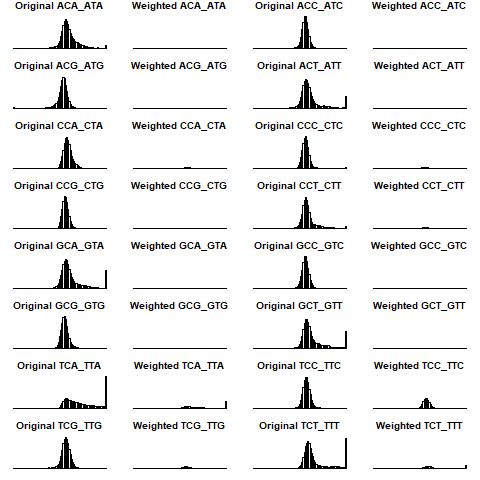
\includegraphics{./png.dir/hist003.png}

Select \(D'_{Pos}\) (\(D'_{Neg}\)) and \(D_{Pos}\) (\(D_{Neg}\)) to
calculate GR and LR This part is included in SigQBiC::SignatureQBiC. We
show this part seperately for tutorial purpose.

\begin{Shaded}
\begin{Highlighting}[]
\NormalTok{QBiC_scores_matrix <-}\StringTok{ }\NormalTok{result}\OperatorTok{$}\NormalTok{QBiC_scores_matrix}
\NormalTok{summaryofscores    <-}\StringTok{ }\NormalTok{result}\OperatorTok{$}\NormalTok{summaryofscores}
\KeywordTok{rm}\NormalTok{(result)}
\NormalTok{pos.sig.QBiC_scores_matrix <-}\StringTok{ }
\StringTok{  }\NormalTok{QBiC_scores_matrix[QBiC_scores_matrix}\OperatorTok{$}\NormalTok{q }\OperatorTok{<}\StringTok{ }\FloatTok{0.1} \OperatorTok{&}\StringTok{ }\NormalTok{QBiC_scores_matrix}\OperatorTok{$}\NormalTok{scores}\OperatorTok{>}\DecValTok{0}\NormalTok{,] }\CommentTok{#select Dpos}


\NormalTok{qvalue.cutoff.score <-}\StringTok{ }\KeywordTok{min}\NormalTok{(pos.sig.QBiC_scores_matrix}\OperatorTok{$}\NormalTok{scores) }\CommentTok{##get the cutoff of QBiC scores based on BH FDR}

\NormalTok{summaryofscores}\OperatorTok{$}\NormalTok{weighted.freq <-}\StringTok{ }
\StringTok{  }\NormalTok{summaryofscores}\OperatorTok{$}\NormalTok{weighted.freq }\OperatorTok{*}\StringTok{ }
\StringTok{  }\KeywordTok{sum}\NormalTok{(summaryofscores}\OperatorTok{$}\NormalTok{frequency)}\OperatorTok{/}\KeywordTok{sum}\NormalTok{(summaryofscores}\OperatorTok{$}\NormalTok{weighted.freq)}
\CommentTok{##Normalize the weighted freqeuencies. After multiplying with signature probability, the weighted frequency is 96 times less than the original frequency. sum(freq) = 96*sum(weighted.freq)}

\NormalTok{summaryofscores.Dpos <-}\StringTok{ }
\StringTok{  }\NormalTok{summaryofscores[summaryofscores}\OperatorTok{$}\NormalTok{scores}\OperatorTok{>}\NormalTok{qvalue.cutoff.score, ] }\CommentTok{##Select Dpos }

\NormalTok{Dpos <-}\StringTok{ }\KeywordTok{rep}\NormalTok{(summaryofscores.Dpos}\OperatorTok{$}\NormalTok{scores, }
\NormalTok{            summaryofscores.Dpos}\OperatorTok{$}\NormalTok{frequency)}

\NormalTok{Dprimepos <-}\StringTok{ }\KeywordTok{rep}\NormalTok{(summaryofscores.Dpos}\OperatorTok{$}\NormalTok{scores, }
                 \KeywordTok{round}\NormalTok{(summaryofscores.Dpos}\OperatorTok{$}\NormalTok{weighted.freq, }\DataTypeTok{digits =} \DecValTok{0}\NormalTok{))}


\NormalTok{summaryofscores.Dneg <-}\StringTok{ }
\StringTok{  }\NormalTok{summaryofscores[summaryofscores}\OperatorTok{$}\NormalTok{scores}\OperatorTok{<}\NormalTok{(}\OperatorTok{-}\NormalTok{qvalue.cutoff.score), ] }\CommentTok{##Select Dneg }

\NormalTok{Dneg <-}\StringTok{ }\KeywordTok{rep}\NormalTok{(summaryofscores.Dneg}\OperatorTok{$}\NormalTok{scores, }
\NormalTok{            summaryofscores.Dneg}\OperatorTok{$}\NormalTok{frequency)}

\NormalTok{Dprimeneg <-}\StringTok{ }\KeywordTok{rep}\NormalTok{(summaryofscores.Dneg}\OperatorTok{$}\NormalTok{scores, }
                 \KeywordTok{round}\NormalTok{(summaryofscores.Dneg}\OperatorTok{$}\NormalTok{weighted.freq, }\DataTypeTok{digits =} \DecValTok{0}\NormalTok{))}

\NormalTok{GR =}\StringTok{ }\KeywordTok{sum}\NormalTok{(Dprimepos)}\OperatorTok{/}\KeywordTok{sum}\NormalTok{(Dpos) }\CommentTok{##GR = 2.952}
\NormalTok{LR =}\StringTok{ }\KeywordTok{sum}\NormalTok{(Dprimeneg)}\OperatorTok{/}\KeywordTok{sum}\NormalTok{(Dneg) }\CommentTok{##LR = 0.058}
\end{Highlighting}
\end{Shaded}

Example of generating one set of random mutations with equal frequency.
We generated 1000 sets of random mutations for statistical test

\begin{Shaded}
\begin{Highlighting}[]
\NormalTok{ResampleMutationFrequency <-}\StringTok{ }\ControlFlowTok{function}\NormalTok{(i)\{}
  \KeywordTok{set.seed}\NormalTok{(i)}
\NormalTok{  resampling.of.mut.type <-}\StringTok{ }\KeywordTok{table}\NormalTok{(}\KeywordTok{sample}\NormalTok{(}\KeywordTok{c}\NormalTok{(}\DecValTok{1}\OperatorTok{:}\DecValTok{96}\NormalTok{),}\DataTypeTok{size=}\KeywordTok{nrow}\NormalTok{(all.possible.twelvemers),}\DataTypeTok{replace=}\NormalTok{T)) }\CommentTok{##Generate mutations based on 96 trinucleotide based with equal frequency}
  
  \KeywordTok{names}\NormalTok{(resampling.of.mut.type) <-}\StringTok{ }\NormalTok{mut.types}
  
\NormalTok{  resampling.of.mut.type <-}\StringTok{ }\NormalTok{resampling.of.mut.type}\OperatorTok{/}\KeywordTok{sum}\NormalTok{(resampling.of.mut.type) }\CommentTok{#Normalize number of mutations to sum of 1}
  \KeywordTok{return}\NormalTok{(resampling.of.mut.type)}
\NormalTok{\}}
\end{Highlighting}
\end{Shaded}

\begin{Shaded}
\begin{Highlighting}[]
\NormalTok{random.mut.freq <-}\StringTok{ }\KeywordTok{data.frame}\NormalTok{(}\KeywordTok{ResampleMutationFrequency}\NormalTok{(}\DecValTok{123}\NormalTok{))}

\KeywordTok{row.names}\NormalTok{(random.mut.freq) <-}\StringTok{ }\NormalTok{mut.types}

\NormalTok{resampling.result <-}\StringTok{ }
\StringTok{  }\KeywordTok{SignatureQBiC}\NormalTok{(}\DataTypeTok{QBiC_score_file_path =}
                  \StringTok{"../data-raw/prediction6mer.Homo_sapiens!M01252_1.94d!Barrera2016!HOXD13_I322L_R1.txt.gz"}\NormalTok{,}
                \DataTypeTok{pvalue_file_path =} 
                  \StringTok{"../data-raw/pval6mer.Homo_sapiens!M01252_1.94d!Barrera2016!HOXD13_I322L_R1.csv.gz"}\NormalTok{,}
\NormalTok{                sig) }
\end{Highlighting}
\end{Shaded}

\end{document}
